
\section{Recent UCVM Applications}

This section showcases research efforts where UCVM has been used to facilitate the creation of discrete velocity meshes based on velocity models that can be used in simulations and research in geosciences.

\subsection{The 2008 Chino Hills Case Study}

On 29 July 2008 the region of southern California and in particular, the greater Los Angeles metropolitan area, was struck by a magnitude \eqmag{w} 5.4 earthquake at 11:42 a.m. The earthquake was the strongest felt in the city since the 1994 Northridge earthquake, but caused no significant damages or fatalities. It provided, nonetheless, an excellent opportunity for earthquake studies because its shaking was recorded on a numerous set of monitoring stations. Since then, UCVM and other SCEC initiatives have used the data during this earthquake as a case study for testing different simulation methods and models. 

Various recent studies done have carefully conducted validations of simulations of the 2008 Chino Hills earthquake with models created using UCVM \citep[e.g.,][]{Olsen_2010_SRL, Taborda_2013_BSSA, Taborda_2014_BSSA}. They have helped test the simulation capabilities of current modeling approaches to predict the ground motion of moderate magnitude earthquakes at low ($<1$~Hz) and moderately (1--4~Hz) and high ($>4$~Hz) frequencies using deterministic and hybrid methods, as well as to propose and test different validation algorithms (goodness-of-fit criteria). 

The latest of these studies \citep{Taborda_2014_BSSA}, in particular, focuses on the validation of simulations of the Chino Hills earthquake using different velocity models, namely CVM-S and CVM-H. This in turn have helped evaluate the differences between the models and their accuracy. The validation performed in this study is based on comparisons with recorded seismograms in over 300 stations scattered throughout the region. The simulation and the models used created with UCVM cover an area of \adomain{180}{135}{km} and go as deep as 62~km. Figure \ref{fig:ch.validation} shows comparisons between the crustal structures of the two models, results of the surface peak ground velocity obtained from the simulations and contour maps of the validation results. The models created for these simulations were built using the etree MPI utilities on NICS's Kraken and NCSA's Blue Waters supercomputer systems employing between XX and YY thousand cores for up to ZZ hours. The sizes of the output (etree) files range between XXX and XXX GB and they comprised between 5 billion and 15 billion octants. \textcolor{red}{(This paragraph needs to be improved.)}

\textcolor{green}{Do the logfiles still exist? Can provide runtimes, resources used (core hours, wallclock), and where it was run.}


% ---------------------------------------------------------------------------------------------
% TEMP FIGURE: Needs to be improved in Illustrator and moved to final PDF dir.
\begin{figure*}[ht!]
	\centering
	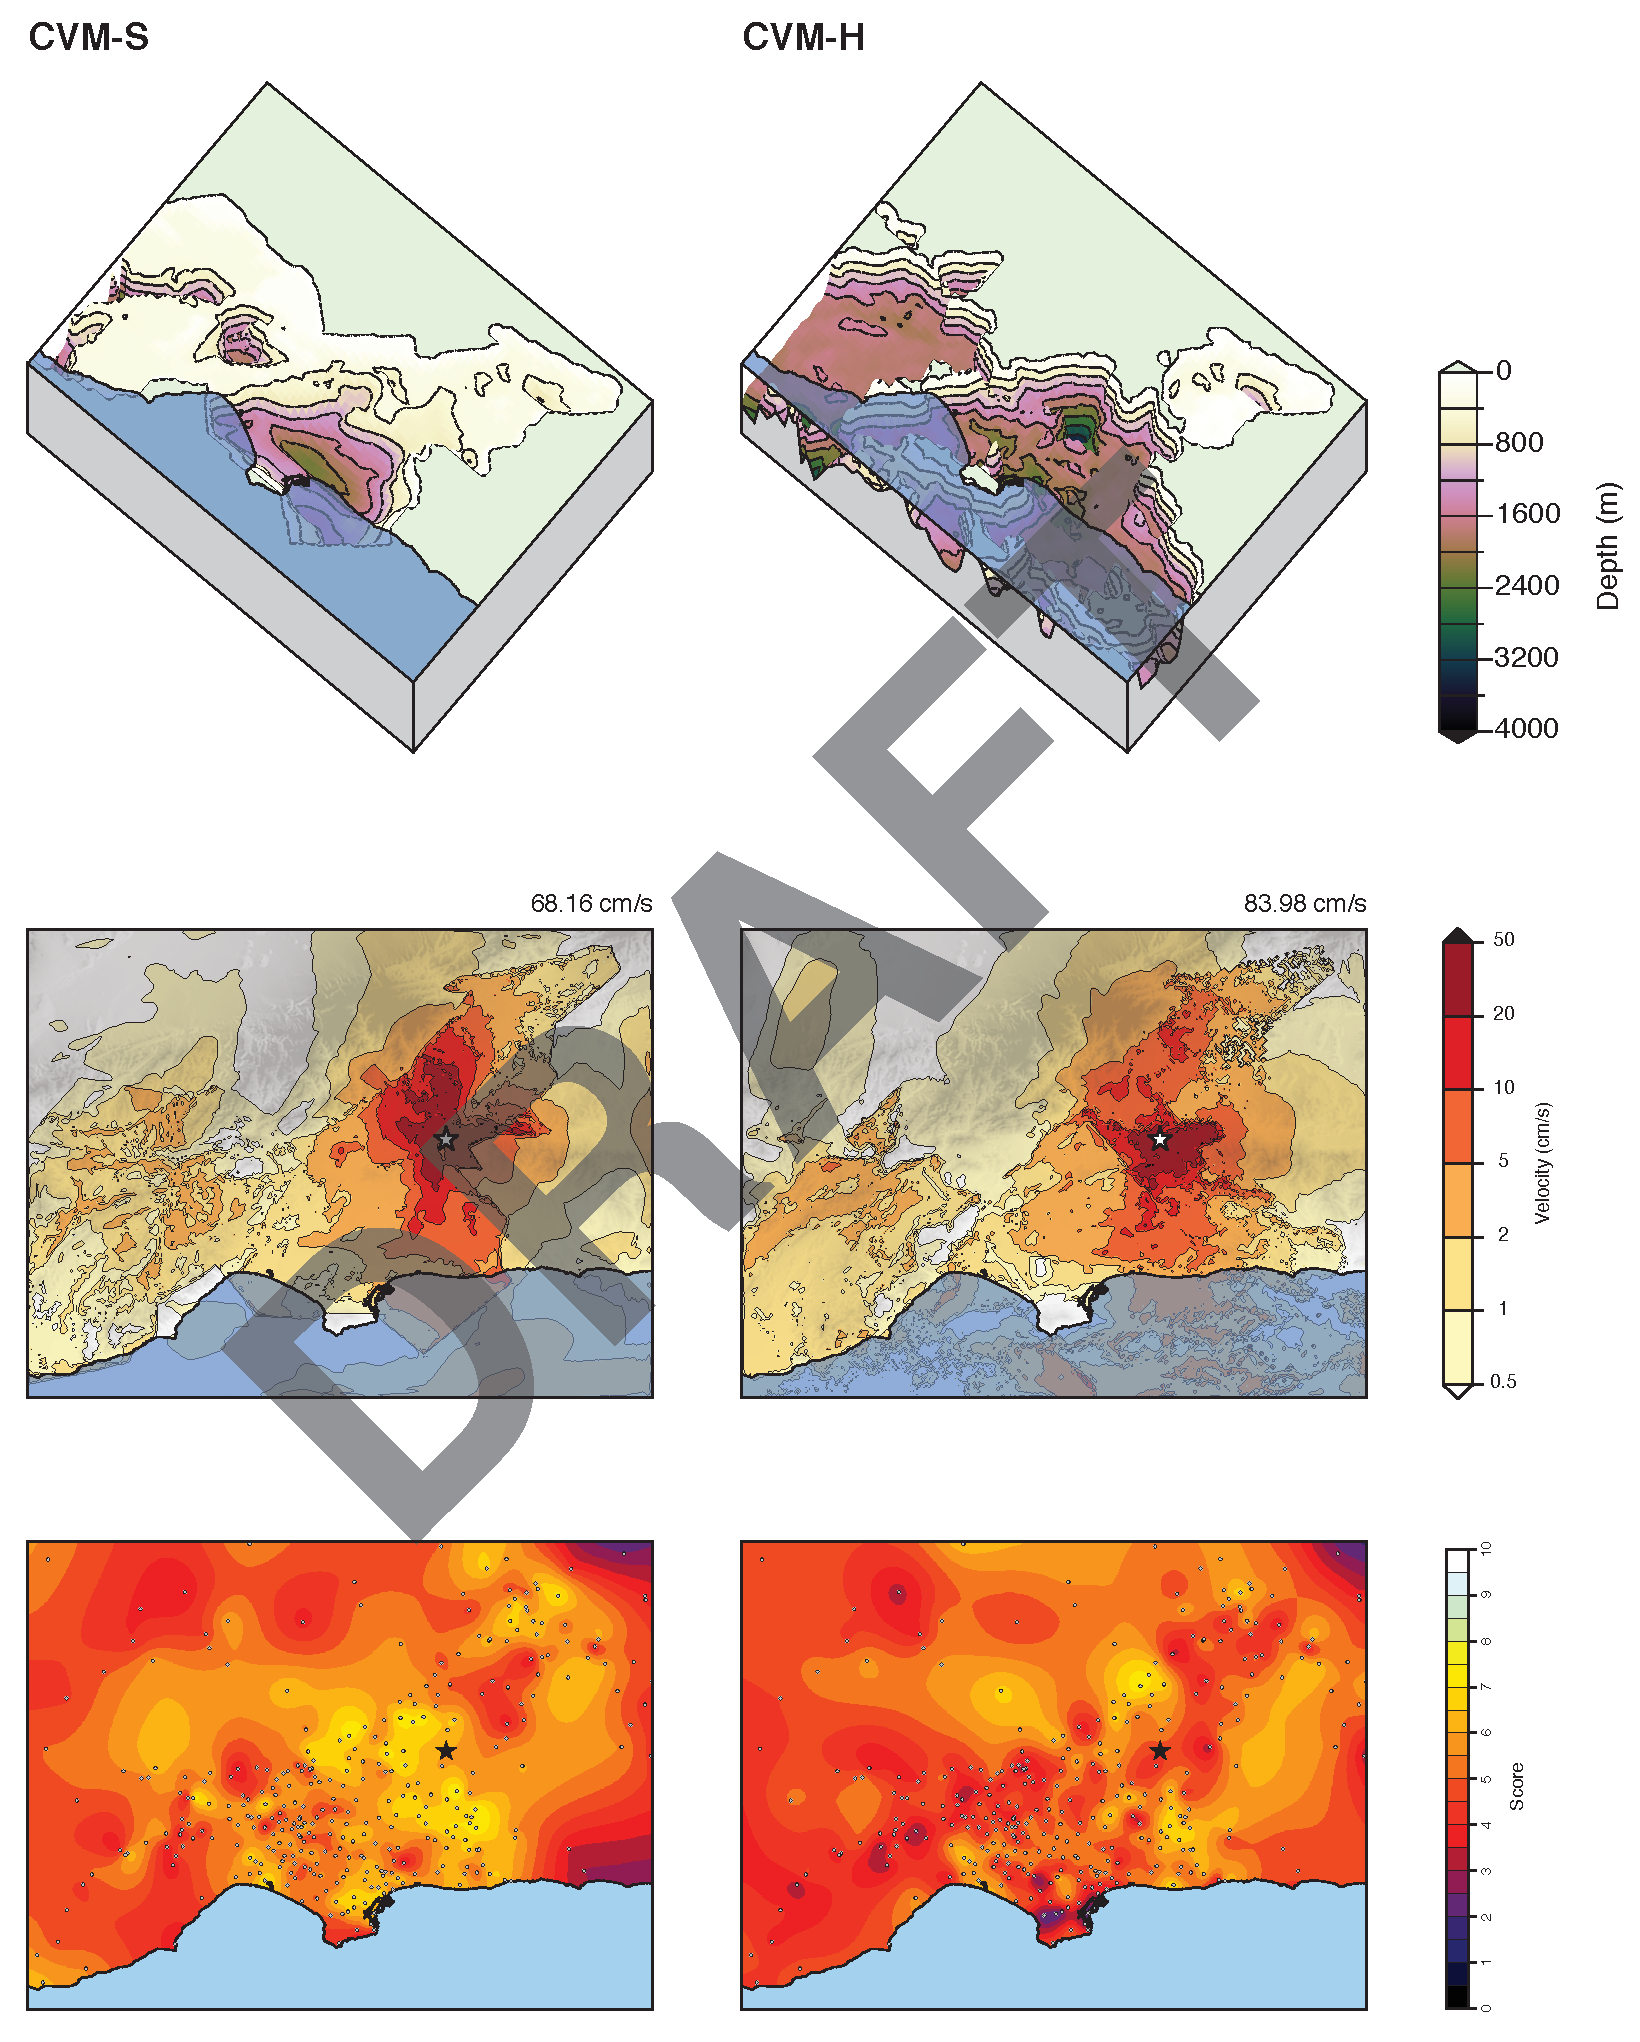
\includegraphics
		[width=0.75\textwidth]
		{figures/raw-pdf/ch-validation}
	\caption{\textcolor{red}{Temporary mock-up figure showing results from Chino Hills validation.}}
	\label{fig:ch.validation}
\end{figure*}
% ---------------------------------------------------------------------------------------------


\subsection{CyberShake}

Probabilistic seismic hazard analysis (PSHA) provides a technique to quantify seismic hazard while taking into account the uncertainties in the model.  SCEC has developed the CyberShake project to perform physics-based PSHA using 3D deterministic wave propagation simulations \citep{Graves_2011_PAG}.  CyberShake performs PSHA by simulating a tensor-valued wavefield of Strain Green Tensors, and then using seismic reciprocity to calculate synthetic seismograms for over 400,000 events per site of interest \citep{Zhao_2006_BSSA}.  These seismograms are processed to obtain intensity measures, which are then combined with probabilities from an earthquake rupture forecast to produce a PSHA hazard curve.  Hazard curves for hundreds of sites can be combined into a hazard map, representing the seismic hazard across a region.

One of the key inputs to CyberShake is the velocity model, which serves as input to the Strain Green Tensor calculation.  Initially CyberShake was developed using custom wrappers for the CVM-S and CVM-H velocity models.  This added complexity to the CyberShake code base, since specialized interface code was required for each velocity model.

To simplify velocity mesh creation via a single interface, CyberShake transitioned to using UCVM upon its release. As a result, two large CyberShake studies were completed in 2013 \citep{Callaghan_2013_Proc} and 2014.  Each produced 4 hazard maps of the Los Angeles area, requiring the generation of 1144 velocity meshes from UCVM, each with 1.2 billion mesh points.  More importantly, CyberShake has been able to calculate hazard maps for 5 different velocity models in the Los Angeles area.  This has enabled detailed analysis of the impact of the velocity model on seismic hazard.  Through techniques such as averaging-based factorization (ABF), we have been able to quantify velocity model-dependent phenomena such as basin and directivity-basin coupling effects \citep{Wang_2014_BSSA}.  A comparison of CyberShake hazard maps calculated with CVM-S4.26 and CVM-H is shown in Figure \ref{fig:cybershake}.


\begin{figure}[ht!]
    \centering
    \includegraphics
        [width=0.9\columnwidth]
        {figures/pdf/cybershake}
    \caption{CyberShake hazard map, 3 seconds spectral acceleration with a 2\% chance of exceedance in 50 years, of the ratio of CVM-S4.26 to CVM-H v11.9.}
    \label{fig:cybershake}
\end{figure}


\subsection{Delivery of CVM-S4.26}

\textcolor{red}{Tentative. I ignore the level of importance UCVM had on preparing the models for Po and En-Jui's inversions in preparation to obtain CVM-S4.26. I suppose that in any case, the fact that CVM-S-4.26 was produced and included in UCVM is something worth showcasing here. i will need, however, to think harder about how to put it in in a nice way.}

\textcolor{green}{Po didn't use UCVM to construct his original model. However, the success story can be the successful delivery of CVM-S4.26 such that it is now publicly available and can be examined by other scientists.}
